\section{ Detector Level Measurements }
\label{sec:DetectorLevel_Measurement}

Figure \ref{fig:reco_VBS_Enhanced_a} shows the measured detector-level data and predicted detector-level yield for six kinematic observables:
\begin{itemize}
    \item{ invariant mass of the dijet system $[m_{jj}]$},
    \item{ invariant mass of the two $Z$ bosons $[m_{4\ell}]$},
    \item{ transverse momentum of the two tagging jets $[p_{T,jj}]$},
    \item{ transverse momentum of the two $Z$ bosons $[p_{T,4\ell}]$},
    \item{ transverse momentum of the two $Z$ bosons and two tagging jets $[p_{T,4\ell jj}]$}, and 
    \item{ scalar transverse momentum of the two $Z$ bosons and dijet $[s_{T,4\ell jj}]$}.
\end{itemize}
Similarly, Figure \ref{fig:reco_VBS_Enhanced_b} shows the detector-level data and prediction for remaining kinematic observables:
\begin{itemize}
\item{ cosine of the decay angle of the negative lepton of the leading (sub-leading) pair in the pair's rest frame $[\cos \theta^{*}_{\ell 1 (3) \ell 2 (4)}]$},
\item{ signed difference between the azimuthal angle of two jets $[\Delta \phi _{jj}^{signed}]$},
\item{ rapidity difference between two jets $[\Delta y_{jj}]$}, and 
\item{ centrality of the system $[\zeta]$}.
\end{itemize}
For each of these distributions, the measured data (black dot) is compared with the state-of-the-art SM predictions, where the two QCD signal $qqZZjj$ (red) and $ggZZjj$ (blue), and the two MC predicted background, $VVV$ (yellow) and $ttV$ (purple) are \textsc{Sherpa} predictions. The contribution from non-prompt backgrounds (light pink) is estimated using the data-driven method. The $qqZZjj$ electroweak signal is obtained from \textsc{PowhegV2}, and the electroweak production of triboson and two jets ($VZZjj$) is obtained from \textsc{Sherpa}. The vertical-solid error bars on the data points represent the statistical uncertainty in the measured data, and the dashed black band in each bin represents the impact of the total theoretical and experimental uncertainties on the predicted detector-level yields. The impact on the bin yield from the total systematic uncertainties and the statistical precision each ranges from $15$ to $20\%$, depending on the bins and the distributions. 

The lower panel in these distributions shows the ratio of data yields to the total SM predicted yields, which are compatible within the total uncertainties. Some discrepancies are observed for some distributions. For instance, the yield is underpredicted in the second and the third bin of $m_{jj}$ and $m_{4l}$, respectively. However, these differences are statistically insignificant. Moreover, a slight but statistically insignificant asymmetry is also observed in the measured distribution of $\Delta \phi _{jj}^{signed}$, which is expected to be symmetric in the SM. 

A simple chi-squared per degree of freedom ($\chi^2/NDF$) is estimated to quantify whether the measured data agree with the SM prediction. As the data yield is event counts, the $\chi^2/NDF$ is computed using the residual difference in each bin between the unweighted data yield and the weighted MC prediction yield. The respective statistical and systematic uncertainties are also considered in the computation of the $\chi^2/NDF$. The reported values of $\chi^2/NDF$ for each distribution in Figures \ref{fig:reco_VBS_Enhanced_a} and \ref{fig:reco_VBS_Enhanced_b} show statistically good agreement between the measured data and SM predictions. Most values of $\chi^2/NDF$ are all smaller than one suggesting the systematic uncertainties could be overestimated in these distributions. The experimental uncertainties related to physics object reconstruction are estimated in a different phase space than the measurements, possibly contributing to the overestimation of the systematic uncertainties. 

\begin{figure}[!htb]
    \centering
    \begin{subfigure}{.49\textwidth}
        \centering
        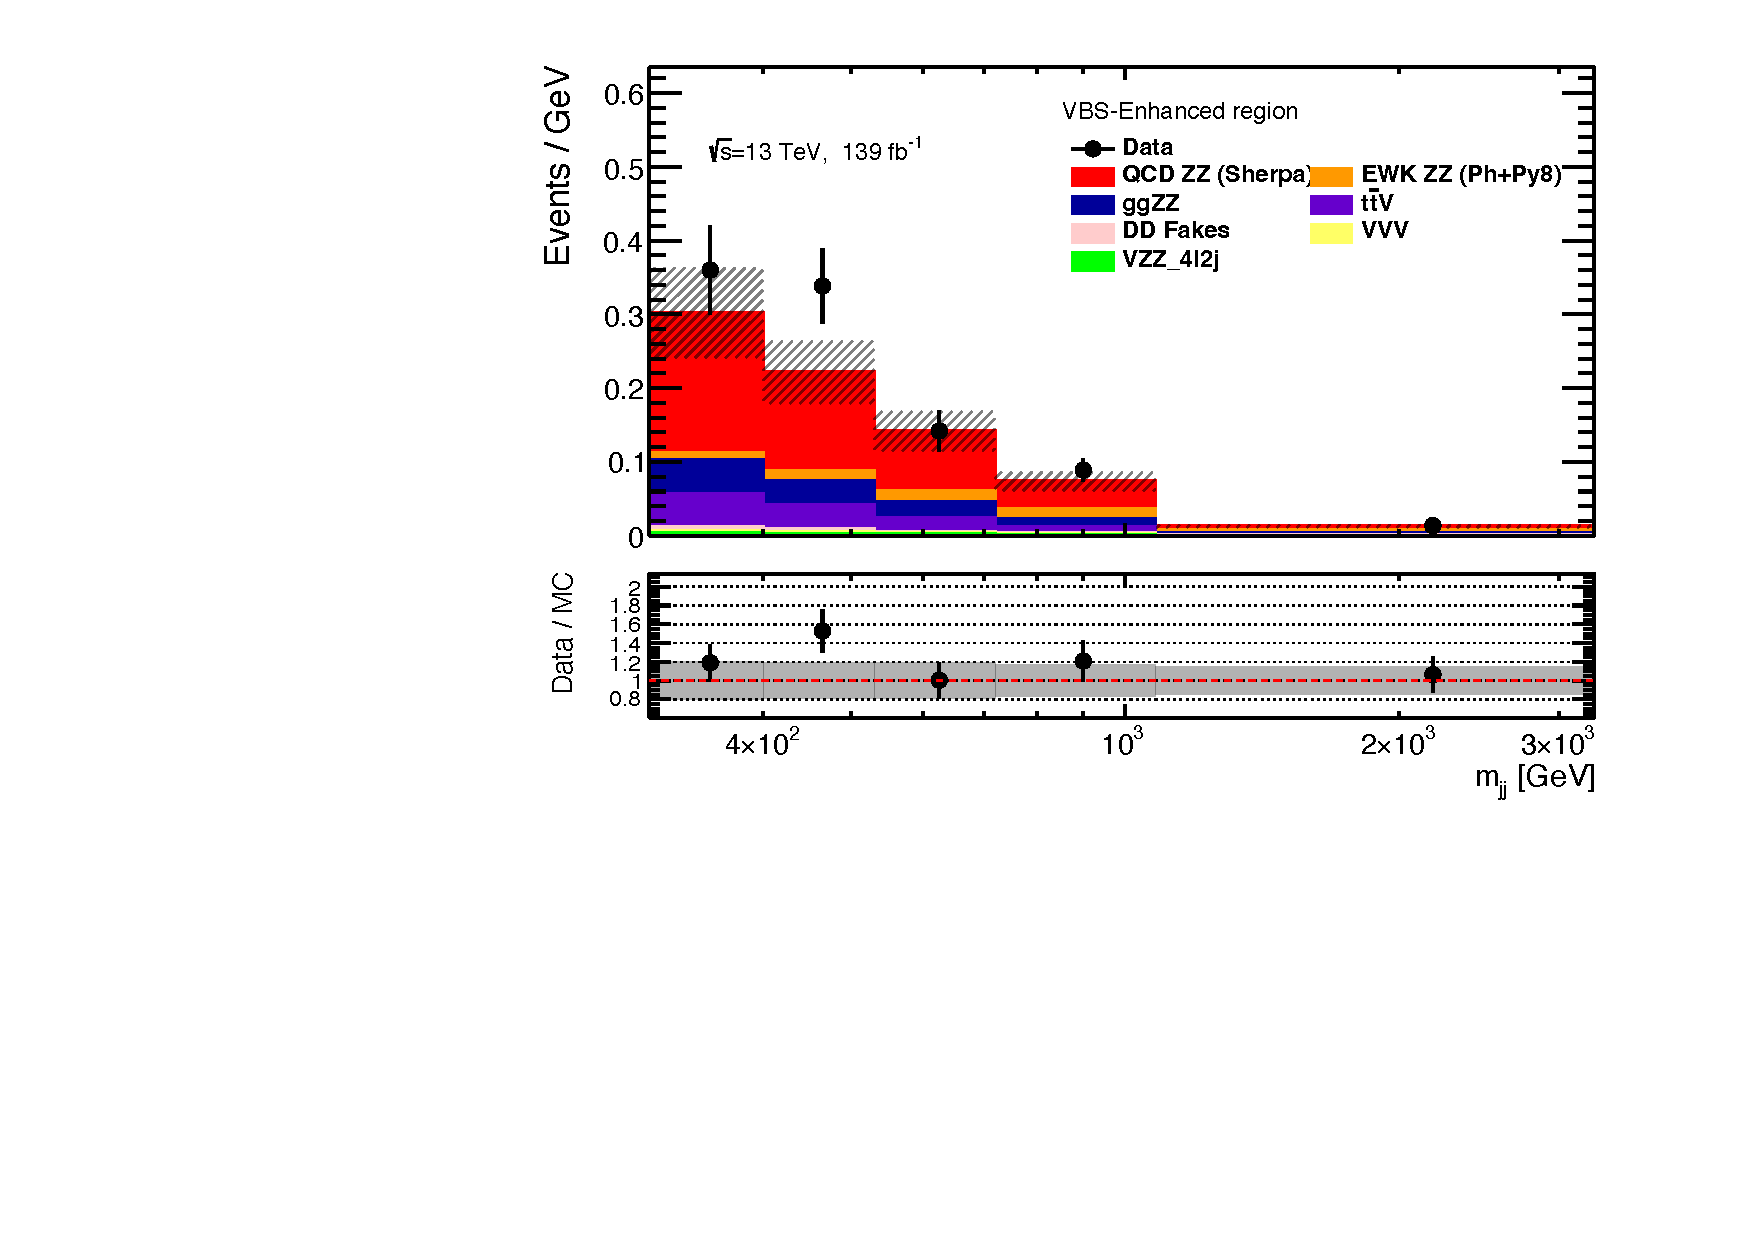
\includegraphics[width=.98\linewidth]{figures/Results/RecoDist_VBSEnhanced/reco_mjj_SR.pdf}
        \caption{ \footnotesize{$m_{jj}$}: $\chi^2/NDF = 0.43$ }
    \end{subfigure}
    \begin{subfigure}{.49\textwidth}
        \centering
        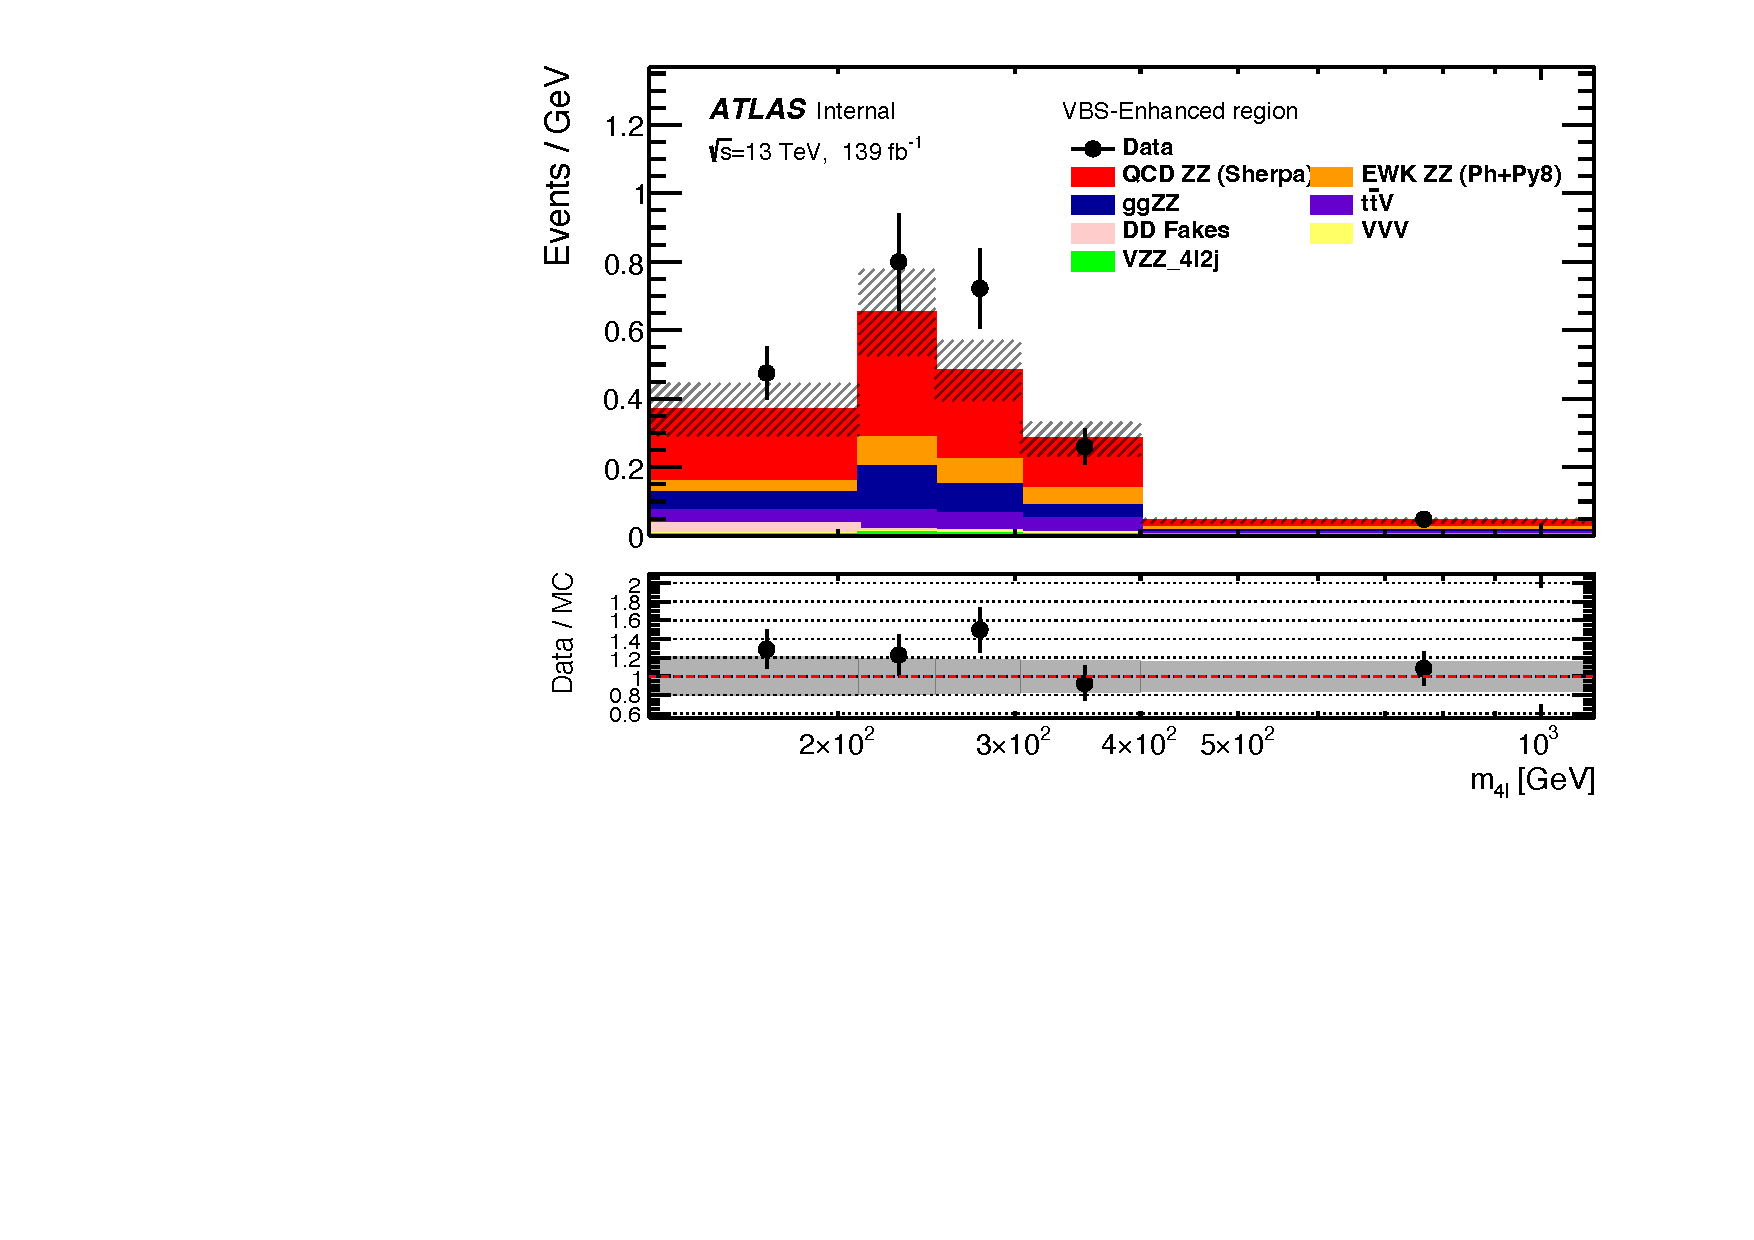
\includegraphics[width=.98\linewidth]{figures/Results/RecoDist_VBSEnhanced/reco_m4l_SR.pdf}
        \caption{ \footnotesize{$m_{4\ell}$ }: $\chi^2/NDF = 0.49$ }
    \end{subfigure}\\
    \begin{subfigure}{.49\textwidth}
        \centering
        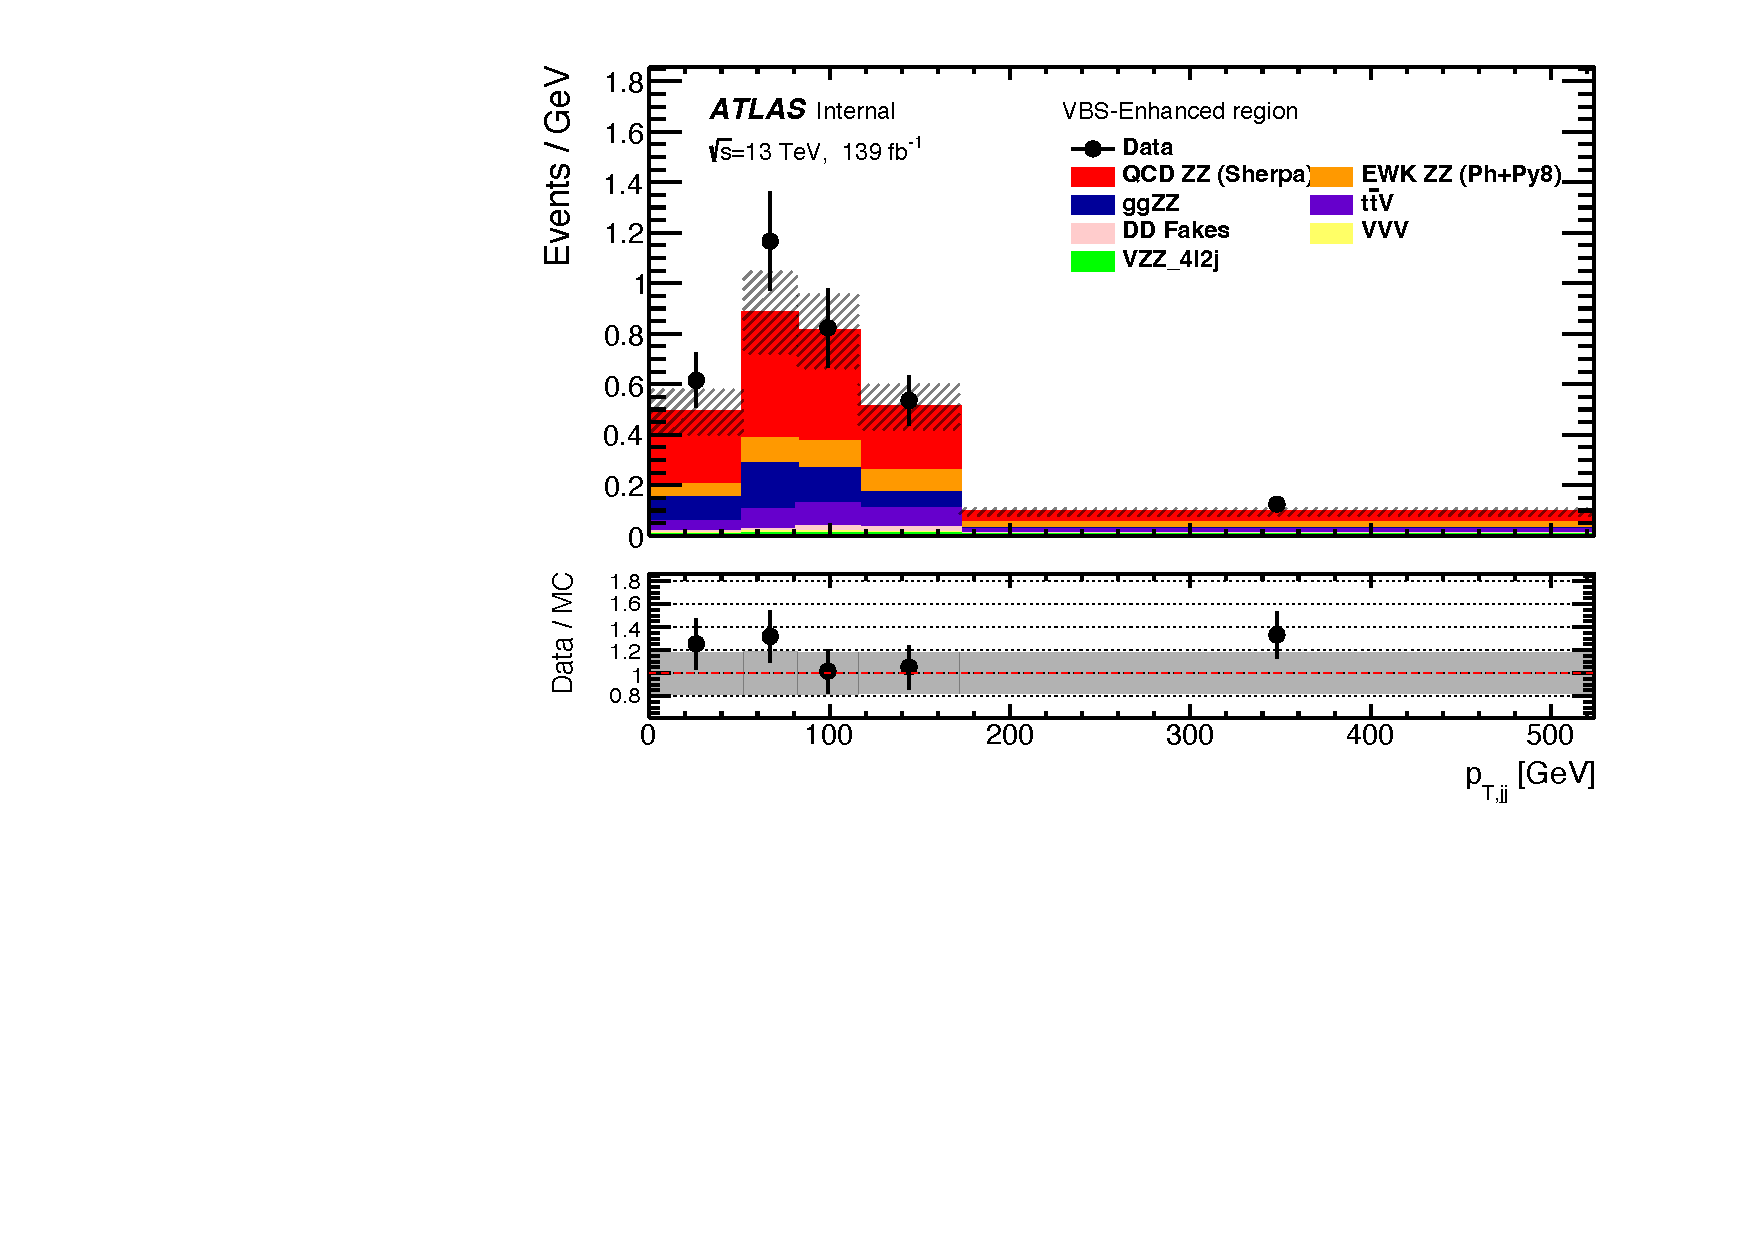
\includegraphics[width=.98\linewidth]{figures/Results/RecoDist_VBSEnhanced/reco_ptjj_SR.pdf}
        \caption{ \footnotesize{$p_{T,jj}$}: $\chi^2/NDF = 0.30$ }
    \end{subfigure}
    \begin{subfigure}{.49\textwidth}
        \centering
        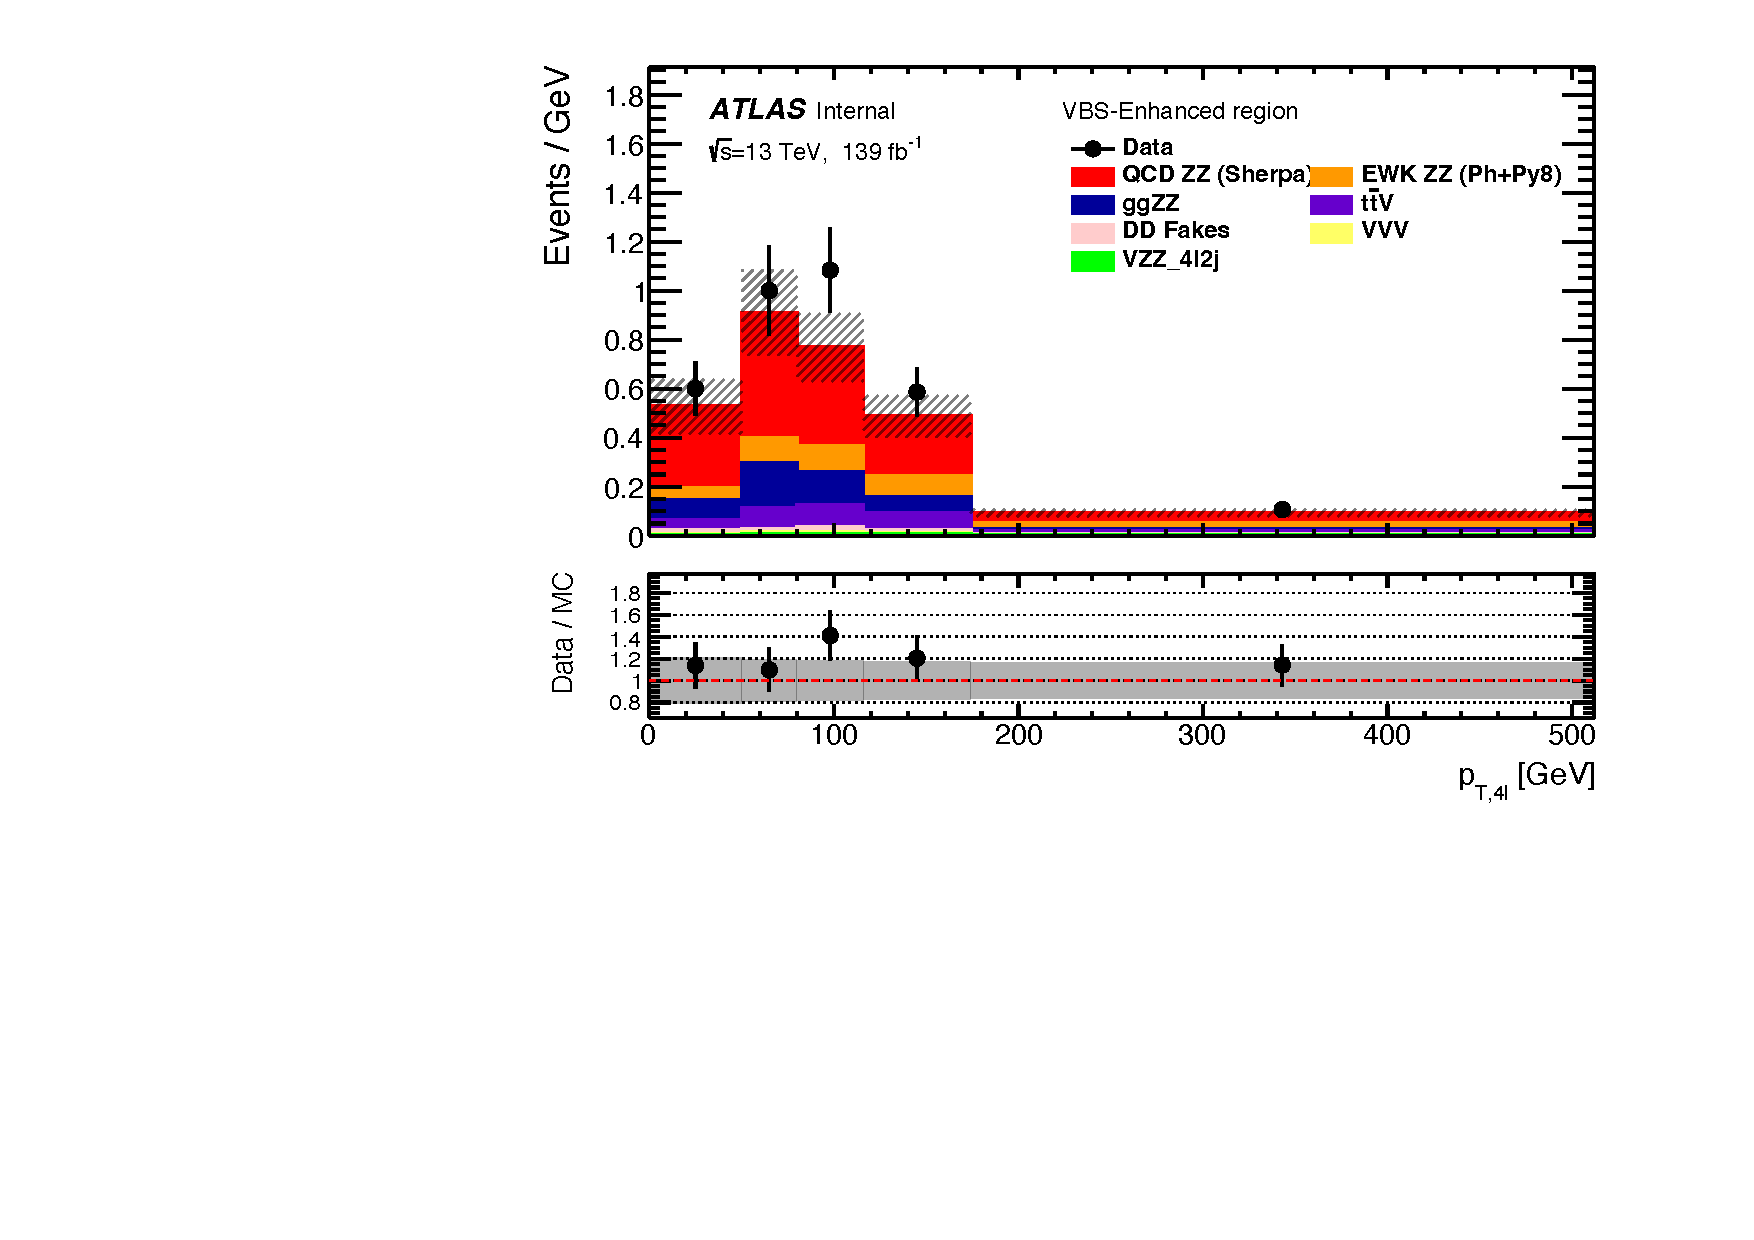
\includegraphics[width=.98\linewidth]{figures/Results/RecoDist_VBSEnhanced/reco_pt4l_SR.pdf}
        \caption{ \footnotesize{$p_{T,4\ell}$ }: $\chi^2/NDF = 0.15$ }
    \end{subfigure}\\
    \begin{subfigure}{.49\textwidth}
        \centering
        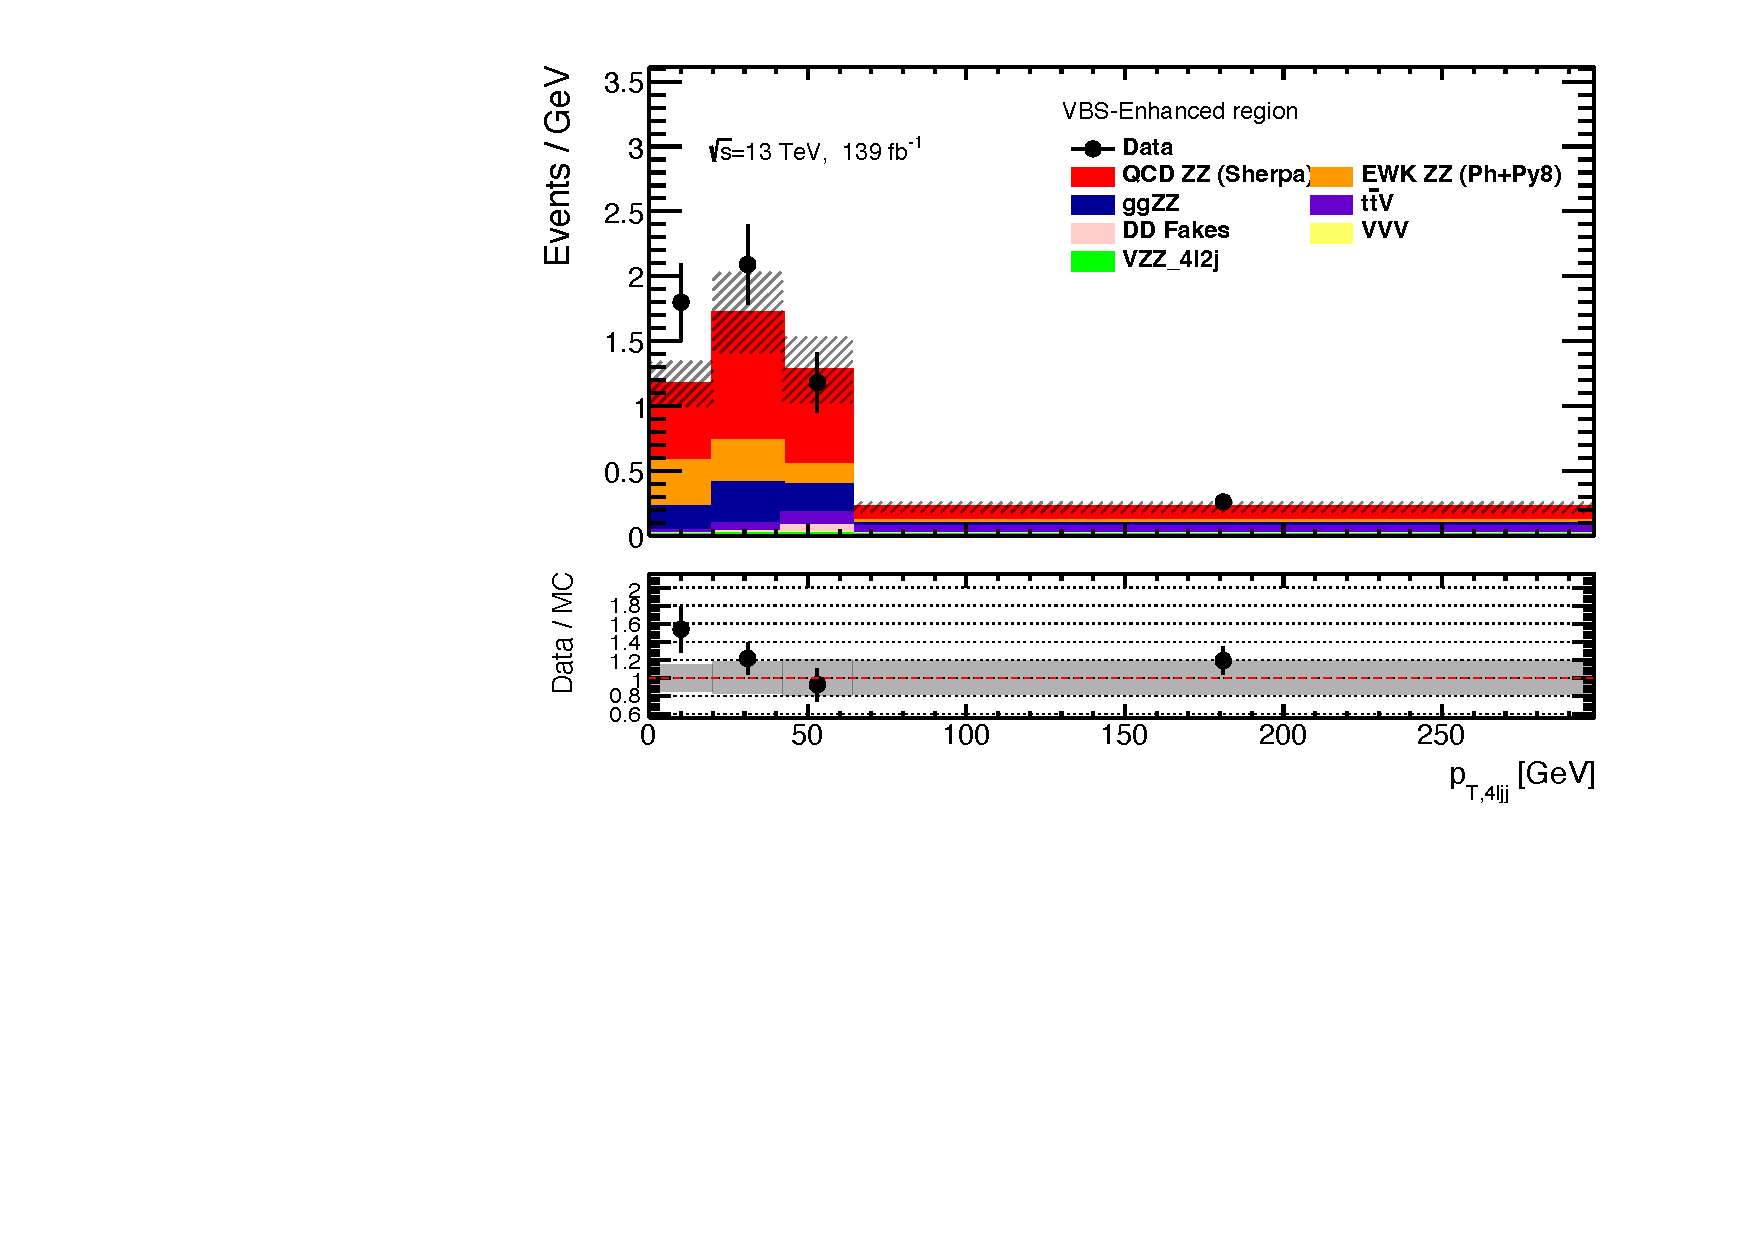
\includegraphics[width=.98\linewidth]{figures/Results/RecoDist_VBSEnhanced/reco_ptzzjj_SR.pdf}
        \caption{ \footnotesize{$p_{T,4\ell jj}$}: $\chi^2/NDF = 0.70$ }
    \end{subfigure}
    \begin{subfigure}{.49\textwidth}
        \centering
        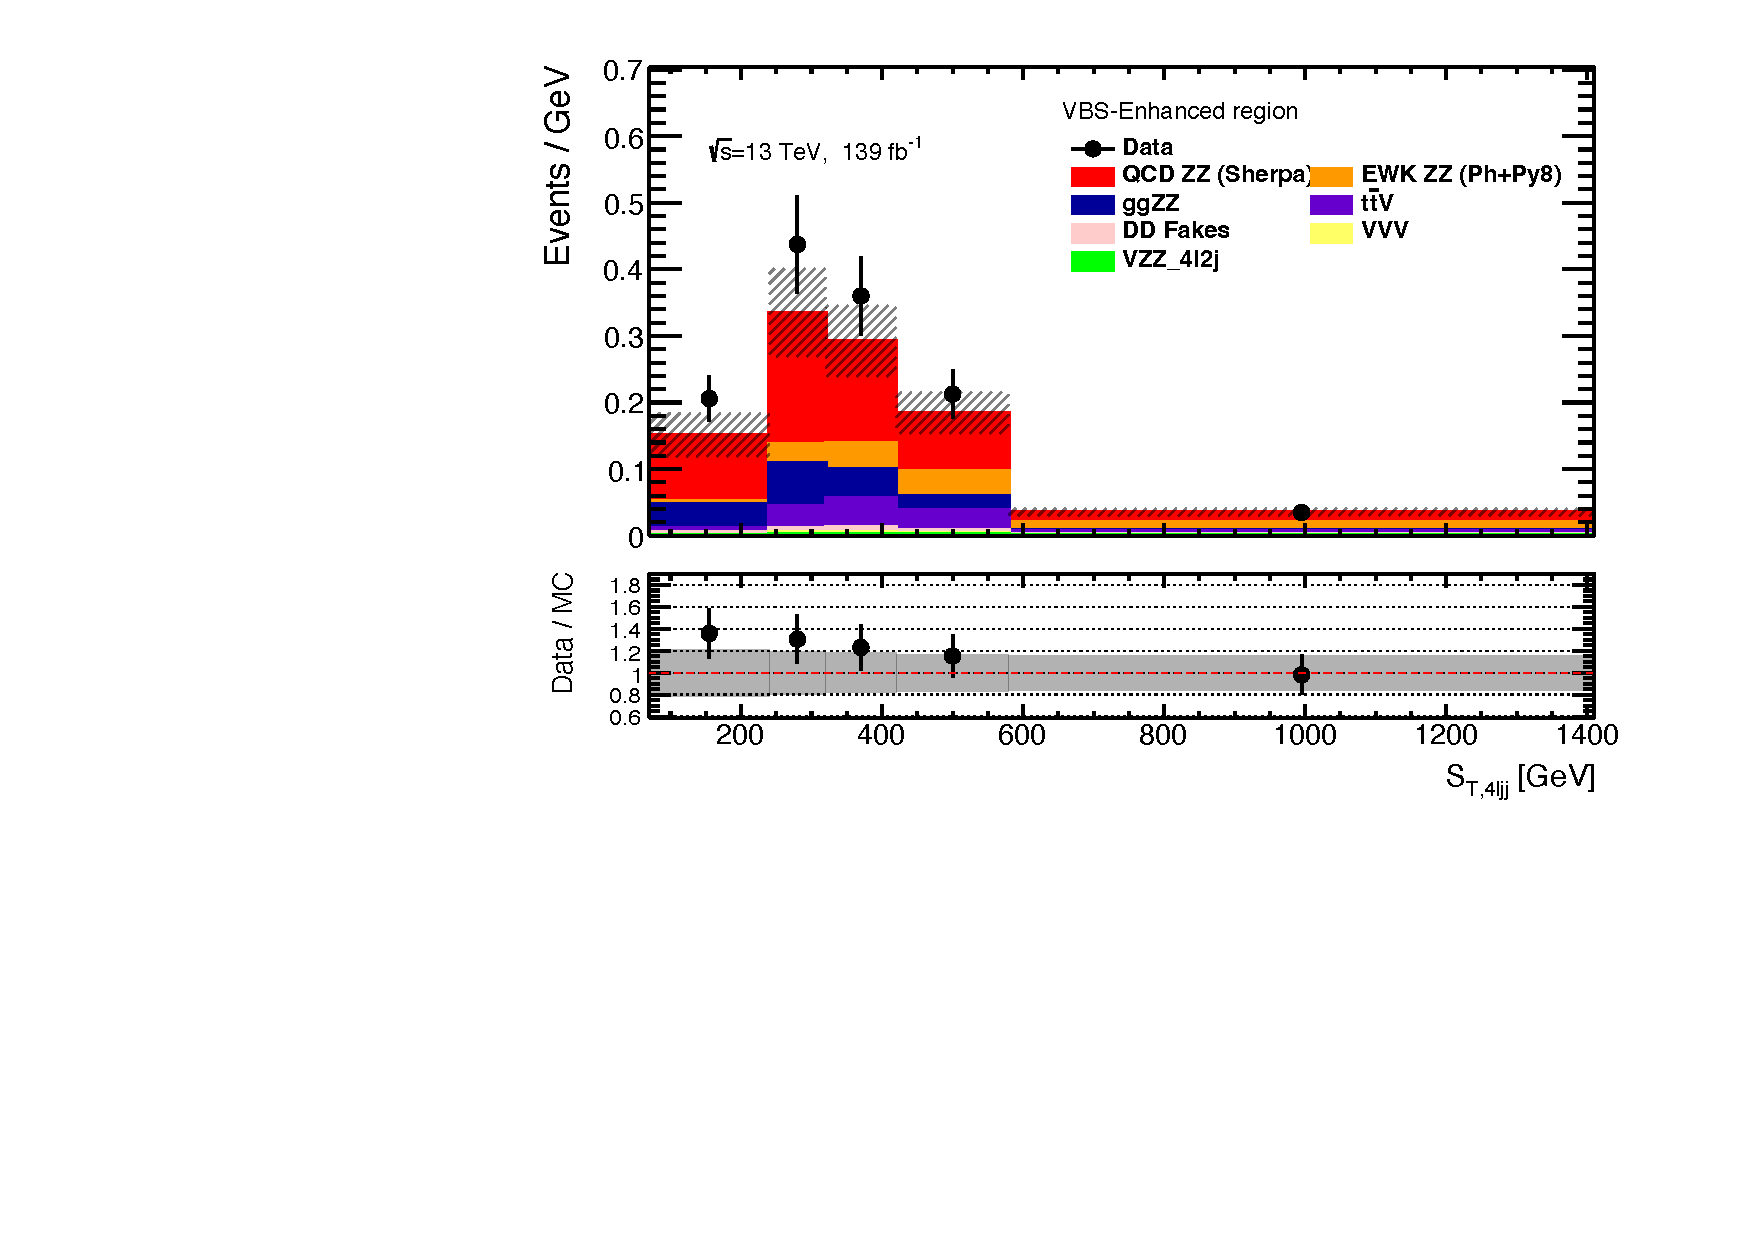
\includegraphics[width=.98\linewidth]{figures/Results/RecoDist_VBSEnhanced/reco_stzzjj_SR.pdf}
        \caption{ \footnotesize{$s_{T, 4\ell jj}$ }: $\chi^2/NDF = 0.24$ }
    \end{subfigure}
    \caption{Detector level distributions in the VBS-Enhanced region.}  \label{fig:reco_VBS_Enhanced_a}
\end{figure}

\begin{figure}[!htb]
    \centering
    \begin{subfigure}{.49\textwidth}
        \centering
        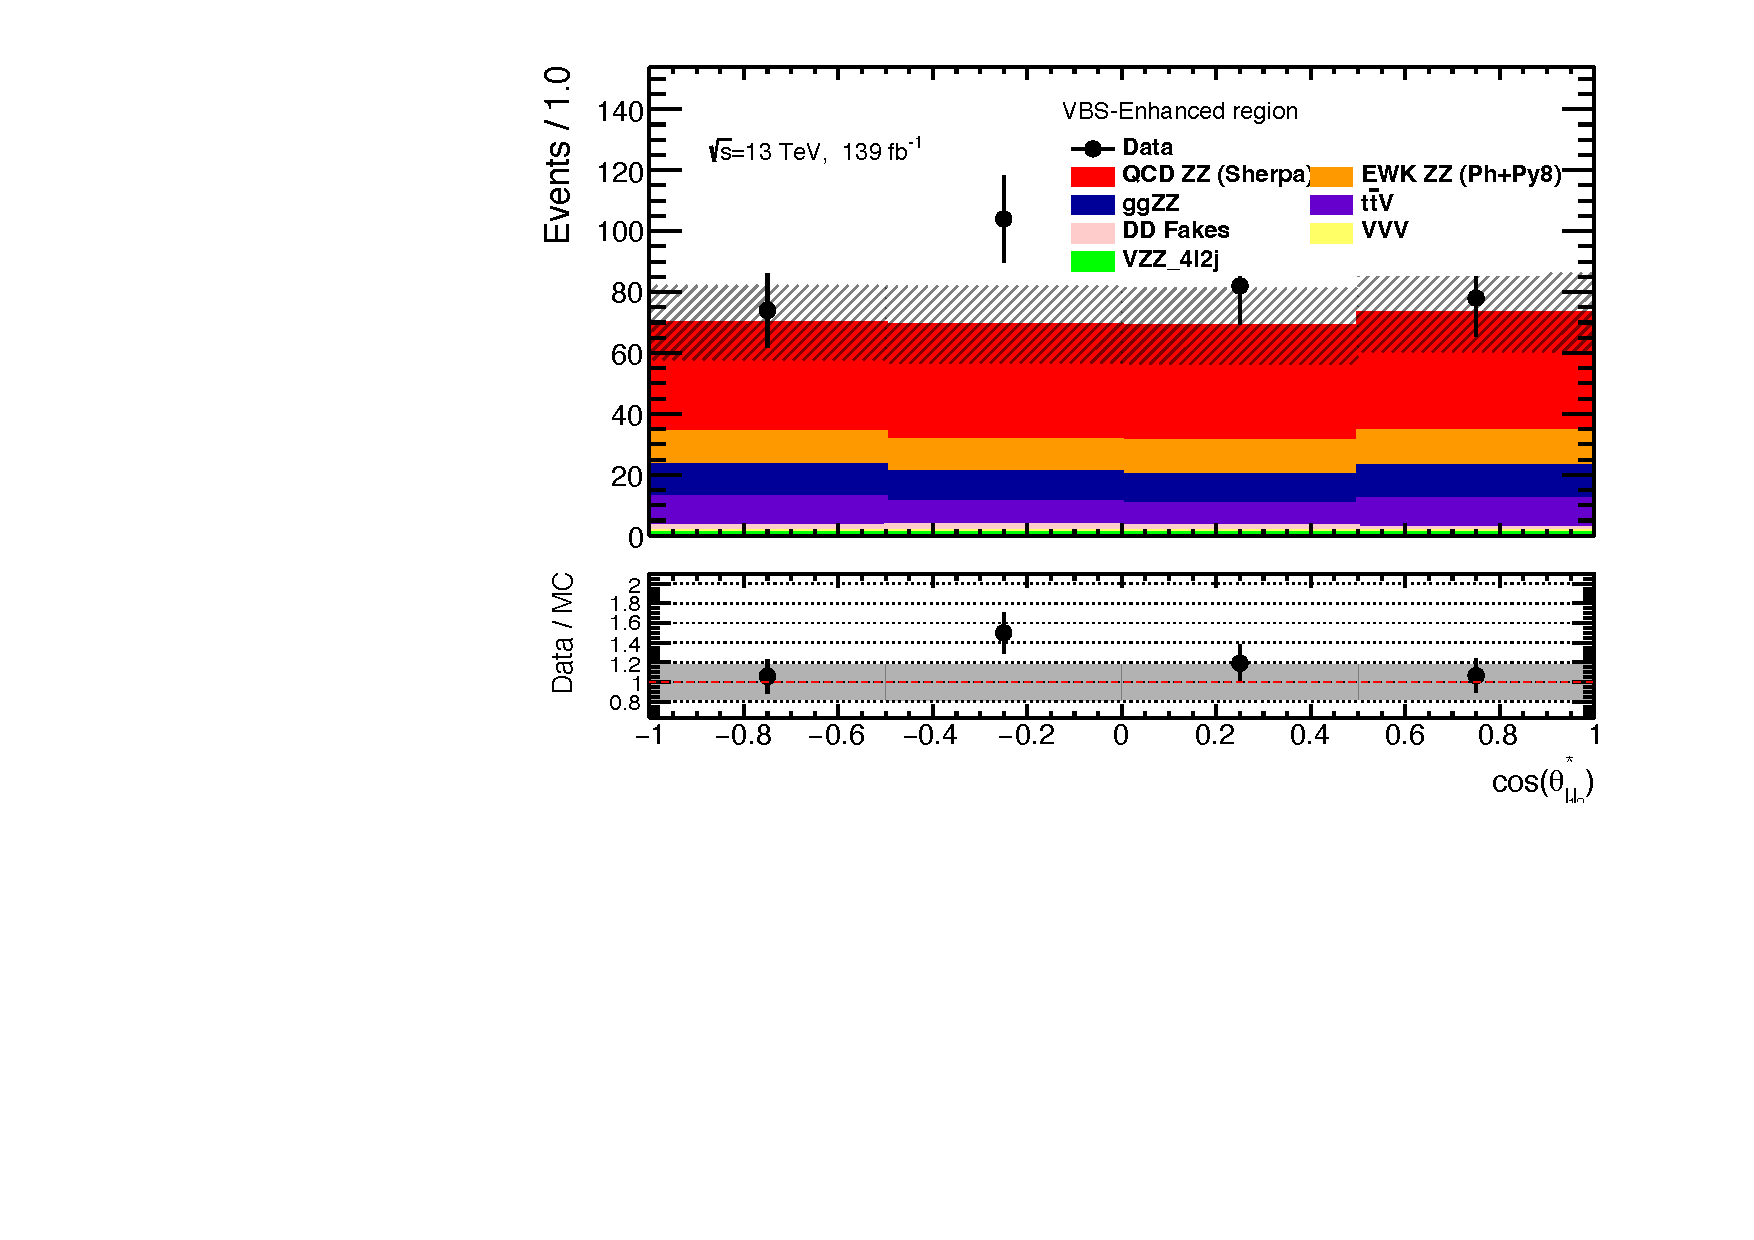
\includegraphics[width=.98\linewidth]{figures/Results/RecoDist_VBSEnhanced/reco_cosThetaStar1_SR.pdf}
        \caption{ \footnotesize{$\cos \theta^{*}_{\ell 1 \ell 2}$}: $\chi^2/NDF = 0.51$ }
    \end{subfigure}
    \begin{subfigure}{.49\textwidth}
        \centering
        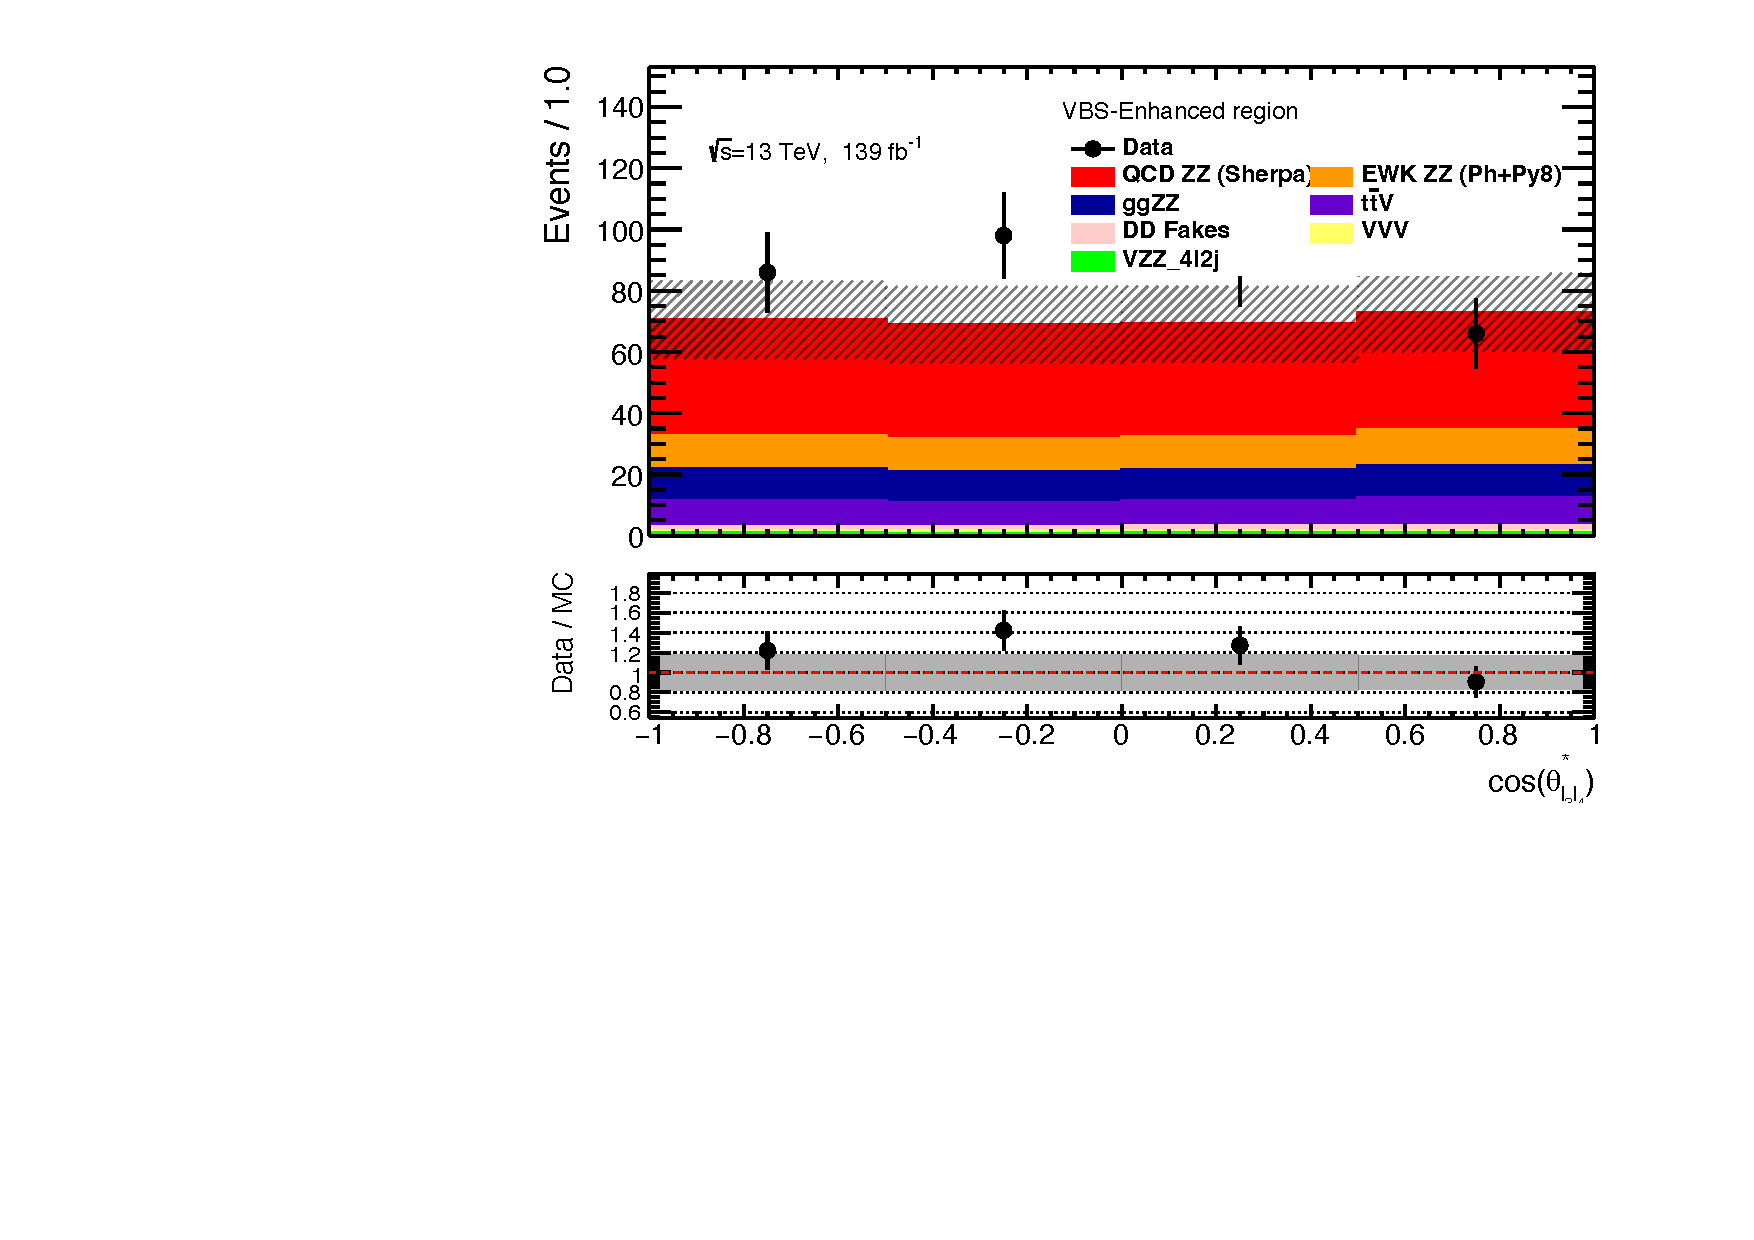
\includegraphics[width=.98\linewidth]{figures/Results/RecoDist_VBSEnhanced/reco_cosThetaStar3_SR.pdf}
        \caption{ \footnotesize{$\cos \theta^{*}_{\ell 3 \ell 4}$ }: $\chi^2/NDF = 0.61$ }
    \end{subfigure}\\
    \begin{subfigure}{.49\textwidth}
        \centering
        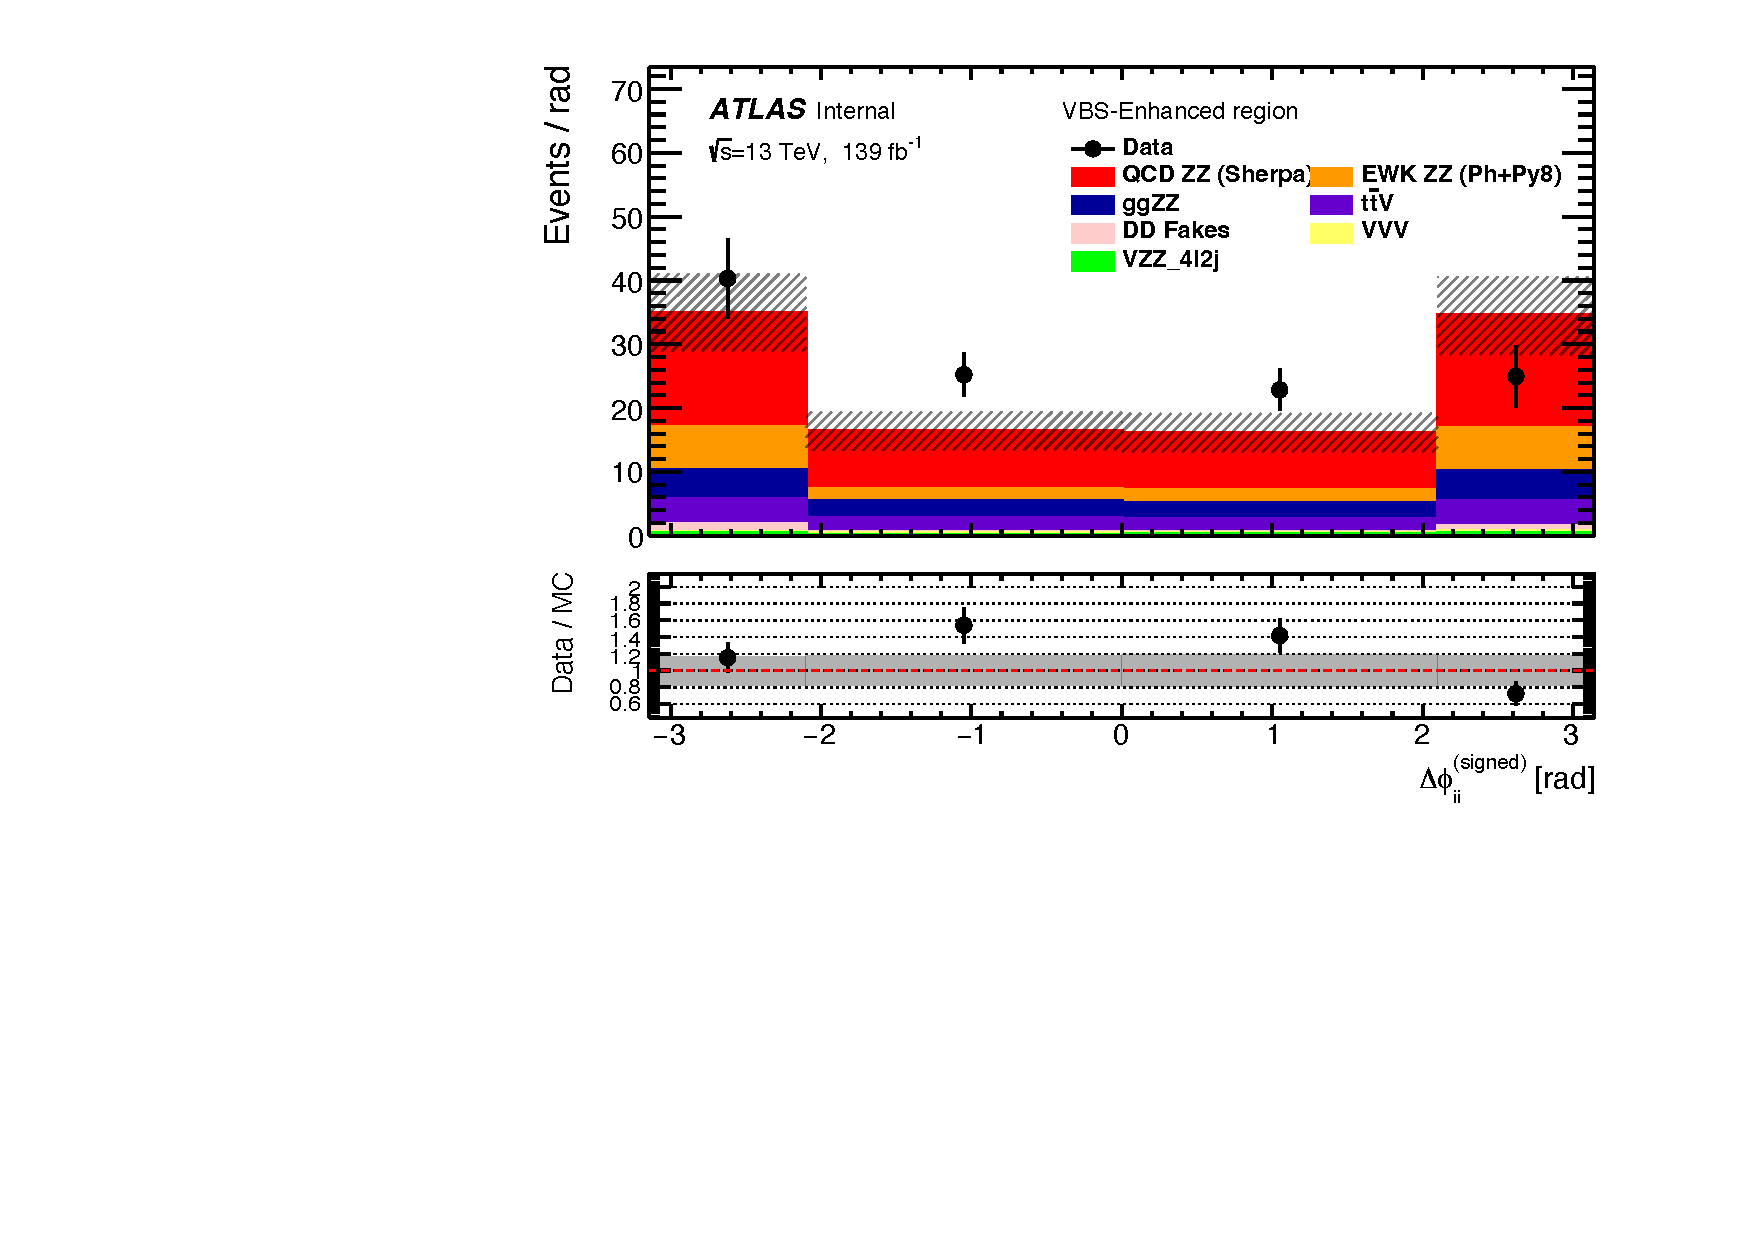
\includegraphics[width=.98\linewidth]{figures/Results/RecoDist_VBSEnhanced/reco_dphi_SR.pdf}
        \caption{ \footnotesize{$\Delta \phi _{jj}^{signed}$ }: $\chi^2/NDF = 1.69$ }
    \end{subfigure}
    \begin{subfigure}{.49\textwidth}
        \centering
        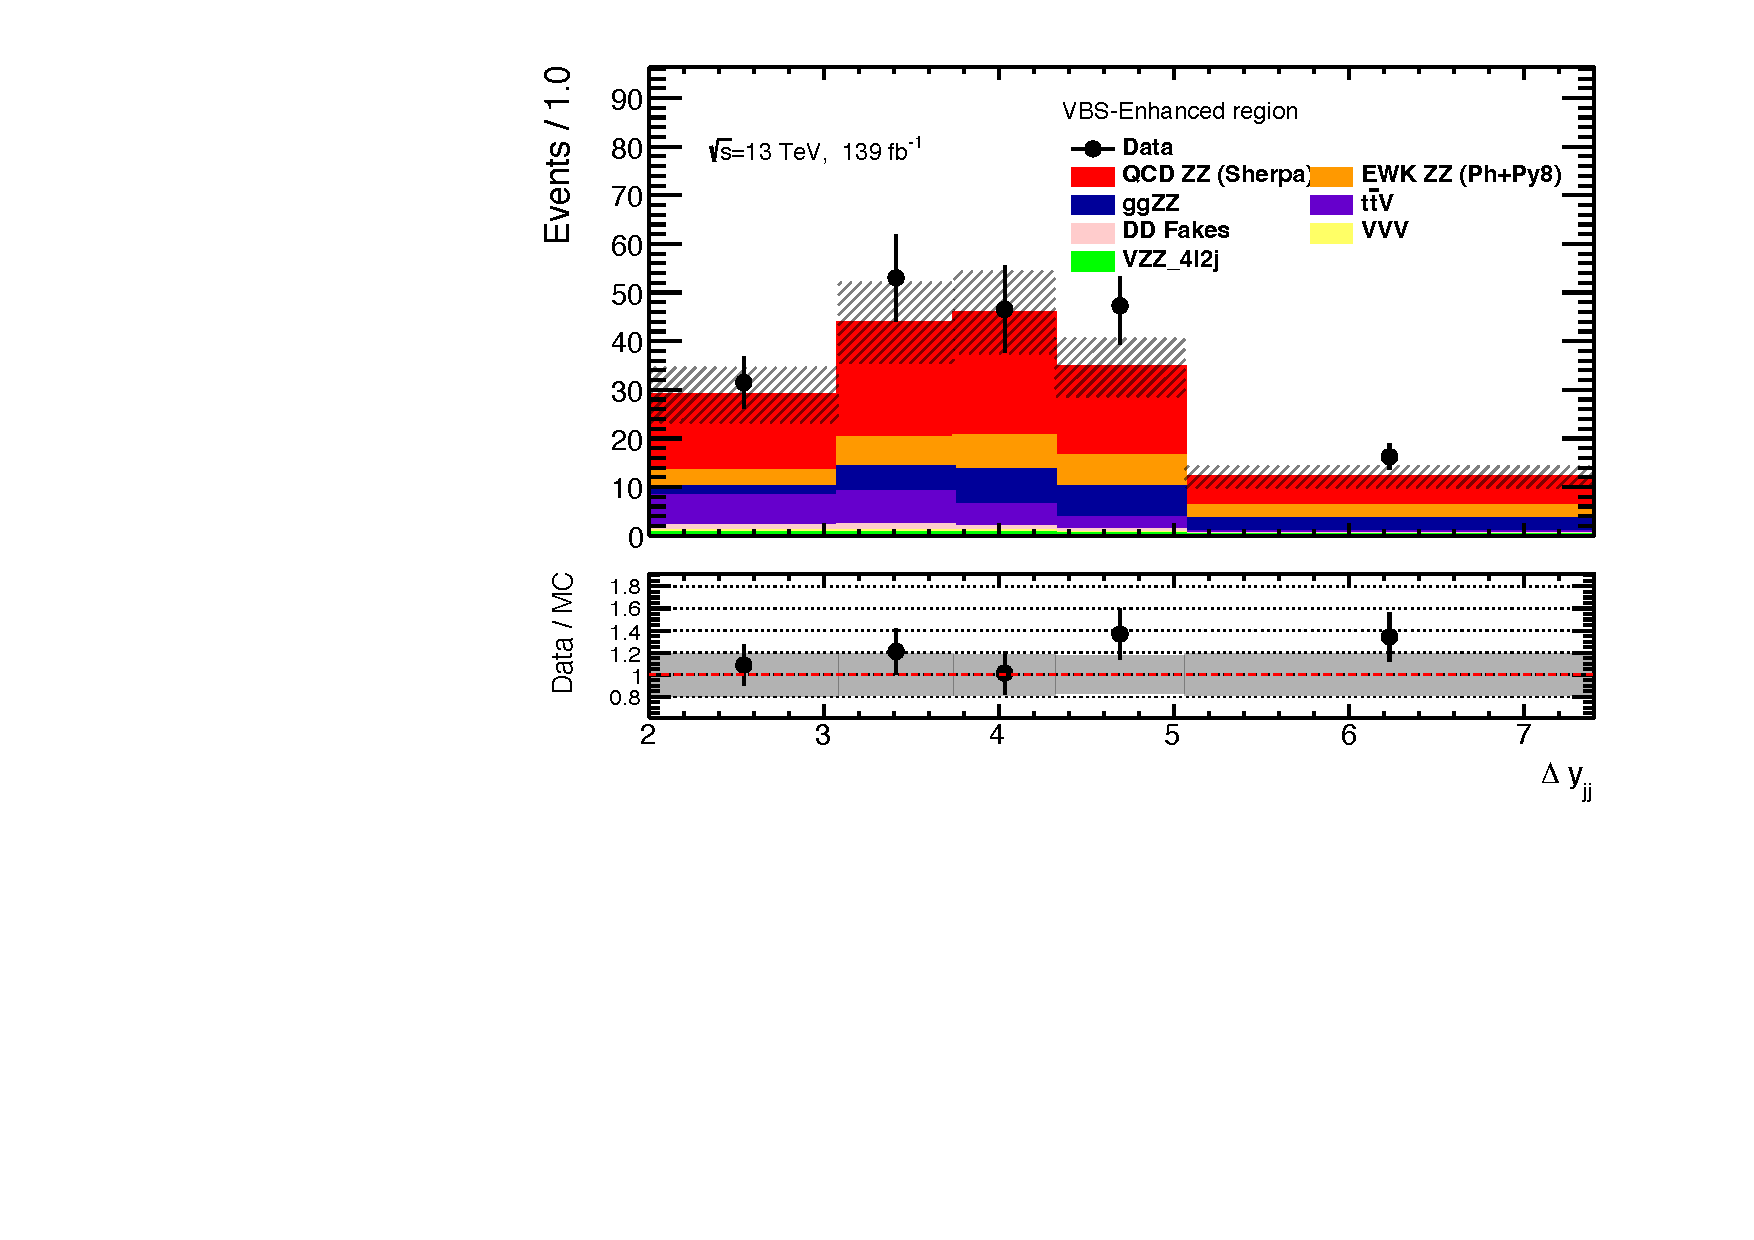
\includegraphics[width=.98\linewidth]{figures/Results/RecoDist_VBSEnhanced/reco_dy_SR.pdf}
        \caption{ \footnotesize{$\Delta y_{jj}$ }: $\chi^2/NDF = 0.26$ }
    \end{subfigure}\\
    \begin{subfigure}{.49\textwidth}
        \centering
        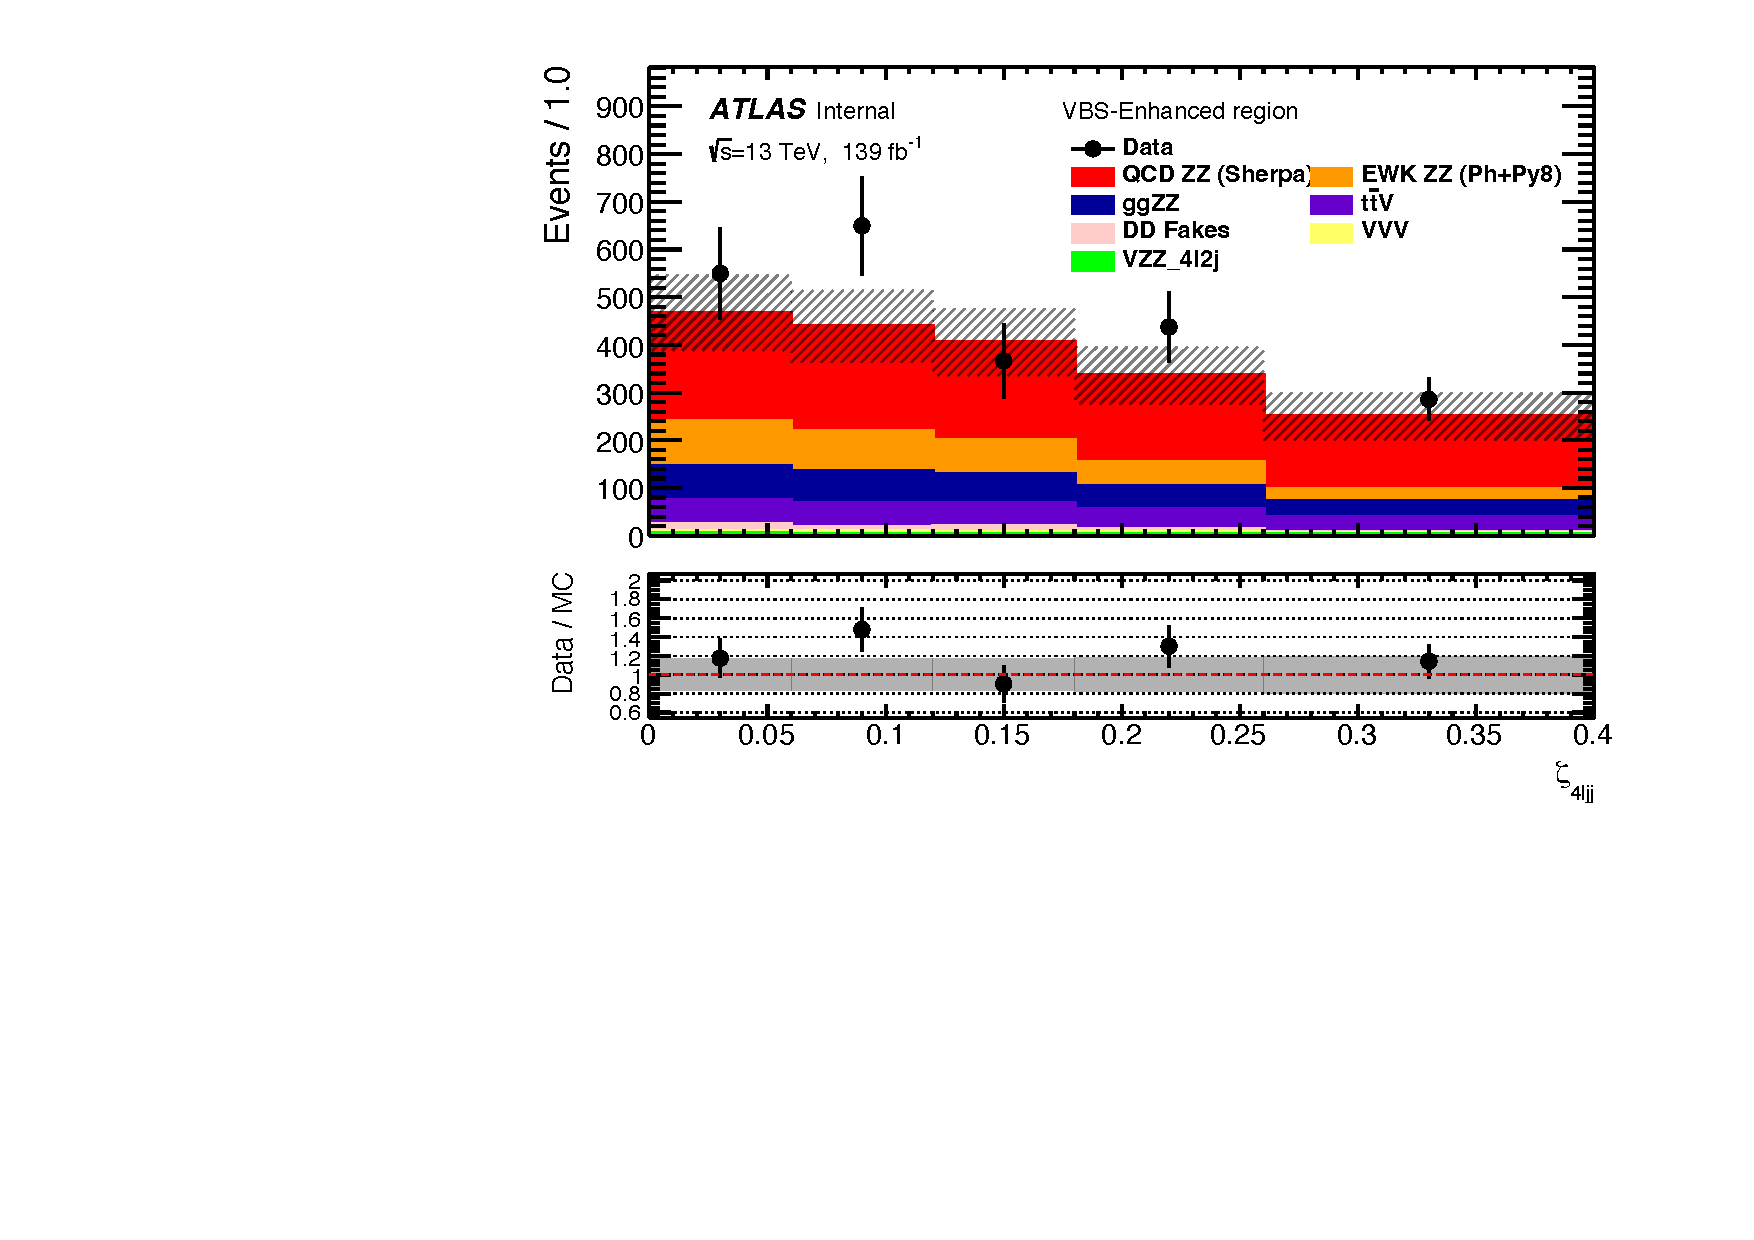
\includegraphics[width=.98\linewidth]{figures/Results/RecoDist_VBSEnhanced/reco_centrality_SR.pdf}
        \caption{ \footnotesize{$\zeta$ }: $\chi^2/NDF = 0.50$ }
    \end{subfigure}
    \caption{Detector level distributions in the VBS-Enhanced region.}  \label{fig:reco_VBS_Enhanced_b}
\end{figure}